\chapter{Resultados e discussões}

\section{Resultados do modelo GRU}
\label{sec:resultados_gru}

A seguir, os resultados alcançados pelo modelo descrita em \ref{fig:gru_pura}:

\begin{table}[H]
\centering
\caption{Resultados do GRU (\textit{N} vs. \textit{V}) na validação}
\label{tab:resultado_cv_gru_validacao}
\begin{tabular}{lcc}
\hline
\textbf{Métrica} & \textbf{Média} & \textbf{Desvio Padrão} \\
\hline
Precisão & 0.8515 & 0.1825 \\
\textit{Recall} & 0.8039  & 0.0795 \\
\textit{F1-Score} & 0.8060 & 0.0760 \\
Acurácia & 0.9640 & 0.0278 \\
\hline
\end{tabular}
\legend{Fonte: Elaborado pelo autor.}
\end{table}

Na tabela \ref{tab:resultado_cv_gru_validacao}, tem-se as métricas médias com seus respectivos desvio padrão na \textit{cross-validação} de cinco \textit{folds}.
Os resultados indicam que o modelo achou aproximadamente 80\% dos casos positivos, com um desvio padrão relativamente baixo, indicando boa estabilidade.
Além disso, a precisão do modelo foi maior que seu \textit{recall}, indicando um perfil mais conservador na classificação. 

A seguir os resultados no treino:

\begin{table}[H]
\centering
\caption{Resultados do GRU (\textit{N} vs. \textit{V}) no treino}
\label{tab:resultado_cv_gru_treino}
\begin{tabular}{lcc}
\hline
\textbf{Métrica} & \textbf{Média} & \textbf{Desvio Padrão} \\
\hline
Precisão & 0.9872 & 0.0121 \\
\textit{Recall} & 0.9782 & 0.0150 \\
F1-Score & 0.9827 & 0.0134 \\
Acurácia & 0.9969 & 0.0024 \\
\hline
\end{tabular}
\legend{Fonte: Elaborado pelo autor.}
\end{table}

Comparando os resultados do treino na tabela \ref{tab:resultado_cv_gru_cnn_treino} com os resultados da validação na tabela \ref{tab:resultado_cv_gru_cnn_validacao},
observa-se um diferença substancial; evidenciando sobreajuste, isto é, o modelo apresentou uma baixa capacidade de generalização para pacientes não vistos.

Esse fenômeno ocorre pois modelos com alta flexibilidade como redes neurais conseguem se ajustar intimamente com os dados de treino
caso eles não sejam representativos da população, eles podem aprender ruído e particularidades dessa amostra ao invés de padrões generalizáveis
No contexto do MIT-BIH, o desbalanceamento das classes pode ter causado isso. Como há poucos exemplos da classe positiva, é fácil para o modelo memorizar
padrões morfológicos e rítmicos das arritmias do conjunto de treino, falhando ao encontrar variações dessas instâncias em pacientes diferentes.

Outra evidência é a diferença entre a acurácia média do conjunto de treino em relação ao conjunto de validação. Observa-se uma 
diferença significantemente menor. Esta métrica é dominada pela classe negativa, indicando que o modelo conseguiu aprender padrões mais generalizáveis
ao ser exposto a mais exemplos dessa classe. 

Diferente da acurácia, as demais métricas são muito mais sensíveis ao desempenho na classe positiva.

O particionamento usado torna a tarefa de generalização mais desafiadora, pois o modelo é avaliado com ECGs não vistos
durante o treino.

Na figura \ref{fig:gru_resultados_por_fold}, está os resultados alcançado pelo modelo em cada \textit{fold} na validação:

\begin{figure}[H]
  \centering
  \caption{Métricas do modelo \ref{fig:gru_pura} por fold \textit{fold}}
   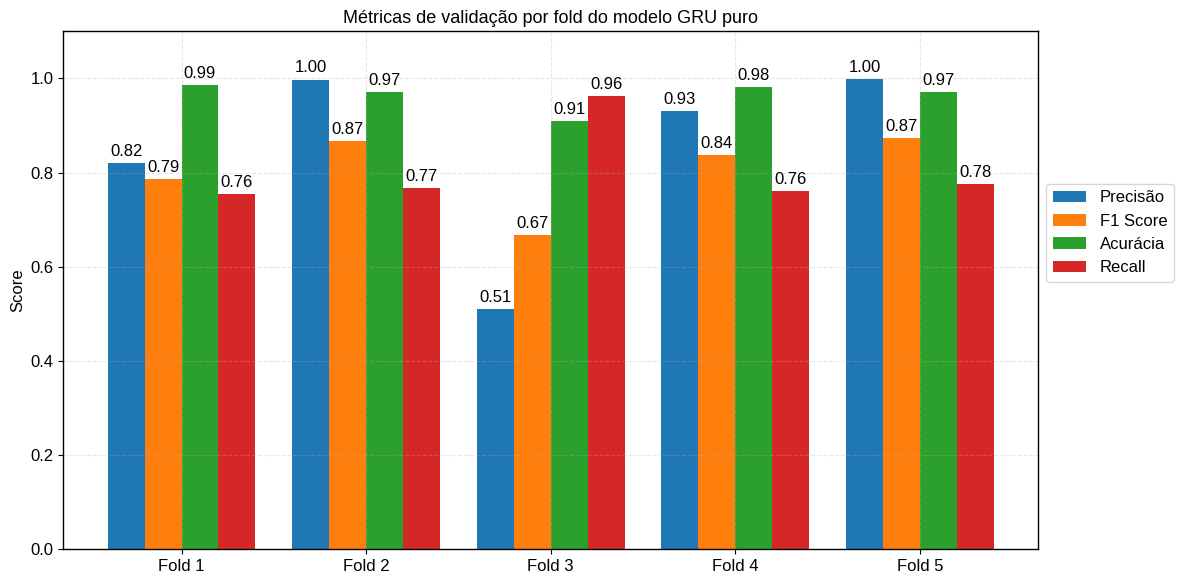
\includegraphics[width=1.0\textwidth]{figuras/modelos_resultados/gru/gru_metricas_por_fold.png} % insere o tikzpicture puro
  \label{fig:gru_resultados_por_fold}
    \legend{Fonte: Elaborado pelo autor.}
\end{figure}

No \textit{fold} três, o modelo obteve sua menor precisão, aproximadamente 0,51 porém obteve um alto \textit{recall}, aproximadamente 0,96.
Essa discrepância sugere que neste \textit{fold}, havia batimentos normais que fugiam do padrão aprendido no treino, fazendo com que o modelo
confundisse eles com batimentos da classe V. Nos demais \textit{folds}, a precisão foi maior que o \textit{recall}, sugerindo a presença 
de arritmias com características mais sutis, que fizeram com que o modelo as confundissem com batimentos normais.

Considerando o \textit{f1-score}, o terceiro \textit{fold} foi eleito o pior. Como o \textit{fold} cinco empatou com o segundo por 
esse mesmo critério, como desempate, aquele com o maior \textit{recall}, o quinto, foi considerado o melhor. 

Na figura \ref{fig:matriz_confusao_melhor_fold_gru}, está a matriz de confusão do modelo em seu melhor \textit{fold}:

\begin{figure}[H]
  \centering
  \caption{Matriz de confusão do modelo \ref{fig:gru_pura} em seu melhor \textit{fold}}
   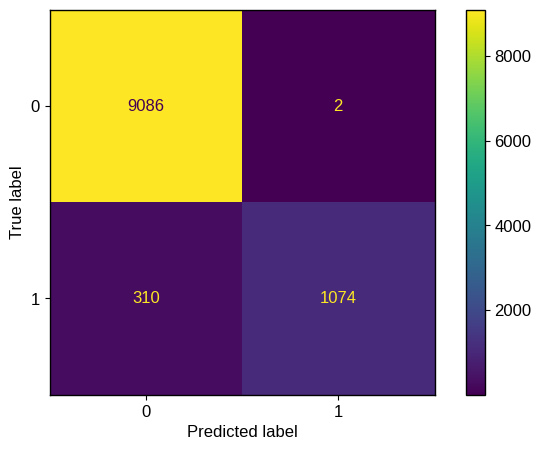
\includegraphics[width=0.7\textwidth]{figuras/modelos_resultados/gru/matriz_confusao_melhor_fold_gru_alt.png} % insere o tikzpicture puro
  \label{fig:matriz_confusao_melhor_fold_gru}
    \legend{Fonte: Elaborado pelo autor.}
\end{figure}

Na matriz, é possível ver o desbalanceamento das classes. Neste \textit{fold}, o número de sequencias pertencentes a classe
negativa é 9.088, enquanto que 1.384 pertencem a positiva; ou seja, aproximadamente, 13,21\% de todas as sequencias são
da classe positiva. 

A maioria dos erros cometidos são de falsos negativos; o modelo classificou 310 sequencias arrítmicas como normais e 
apenas duas normais como arrítmicas. Algo que já era evidenciado no gráfico \ref{fig:gru_resultados_por_fold}, pois 
sua precisão foi maior que seu \textit{recall}.

%O modelo achou 78\% das arritmias. Porém no pior, como pode ser visto na figura \ref{fig:ap_gru_pior_fold}, o modelo conseguiu achar 96\% das arritmias.
Na figura \ref{fig:matriz_confusao_pior_fold_gru}, é dada a matriz de confusão no pior \textit{fold}

\begin{figure}[H]
  \centering
  \caption{Matriz de confusão do modelo \ref{fig:gru_pura} em seu pior \textit{fold}}
   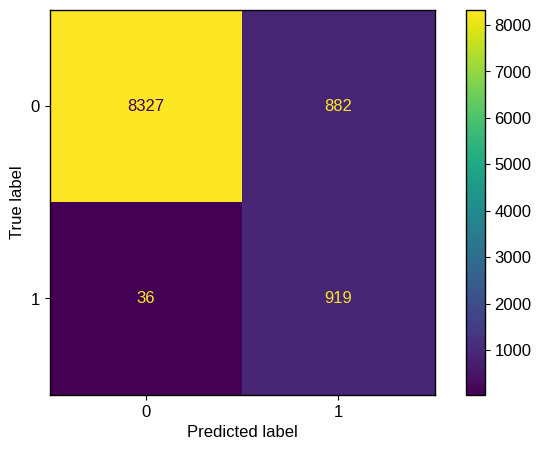
\includegraphics[width=0.7\textwidth]{figuras/modelos_resultados/gru/matriz_confusao_pior_fold_gru_alt.png} % insere o tikzpicture puro
  \label{fig:matriz_confusao_pior_fold_gru}
  \legend{Fonte: Elaborado pelo autor.}
\end{figure}

Aqui o desbalanceamento foi mais severo; havia 9.209 classes negativas e 955 classes positivas; 9,39\% aproximadamente. 
Neste \textit{fold}, a situação se inverte: a maioria dos erros foram de falsos positivos, confirmando o que foi visto no 
gráfico \ref{fig:gru_resultados_por_fold}.

%As duas figuras ilustram como o modelo conseguiu aprender melhor a classe negativa do que a classe positiva; evidenciado pelo fato dele confundir
%muito menos negativo com positivo do que o contrário. Um resultado esperado devido a essa ser a classe dominante em todos os \textit{folds}.

A seguir, na figura \ref{fig:roc_cnn_gru_melhor_fold}, a curva ROC no melhor \textit{fold}:

\begin{figure}[H]
  \centering
  \caption{Curva \textit{ROC} modelo \ref{fig:gru_pura} em seu melhor \textit{fold}}
   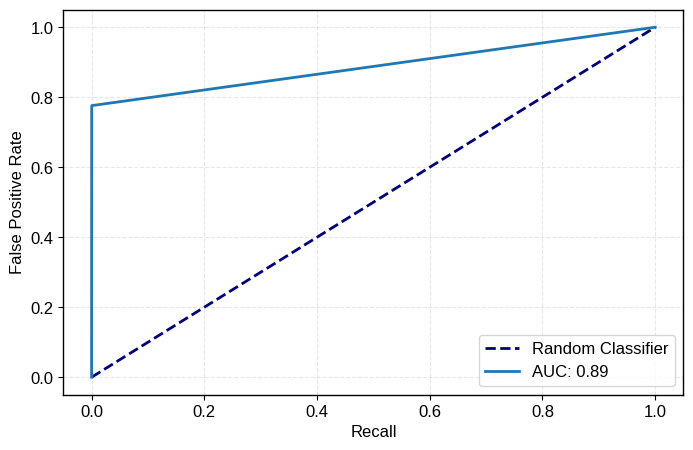
\includegraphics[width=0.7\textwidth]{figuras/modelos_resultados/gru/roc_gru_melhor_fold.png} % insere o tikzpicture puro
  \label{fig:roc_melhor_fold_gru}
  \legend{Fonte: Elaborado pelo autor.}
\end{figure}

Considerando que o \textit{baseline}, um classificador aleatório, tem um \textit{ROC} de 0,5, o melhor foi significantemente melhor.

\begin{figure}[H]
  \centering
  \caption{Curva \textit{ROC} do modelo \ref{fig:gru_pura} em seu melhor \textit{fold}}
   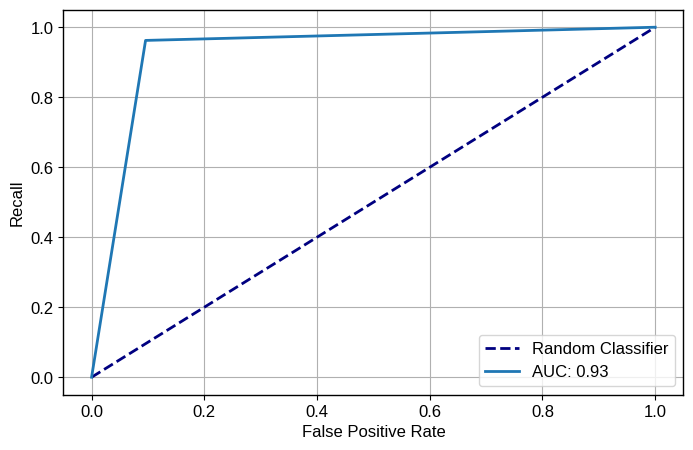
\includegraphics[width=0.7\textwidth]{figuras/modelos_resultados/gru/roc_gru_pior_fold.png} % insere o tikzpicture puro
  \label{fig:roc_pior_fold_gru}
  \legend{Fonte: Elaborado pelo autor.}
\end{figure}

No pior fold, \ref{fig:roc_pior_fold_gru}, o modelo ainda conseguiu manter uma performance satisfatória, com um \textit{ROC} de 0,87. 
Entretanto, devido ao desbalanceamento dos conjuntos, o desempenho pode ser melhor analisado com a curva PR:

\begin{figure}[H]
  \centering
  \caption{Curva precisão vs \textit{recall} do modelo \ref{fig:gru_pura} em seu pior \textit{fold}}
   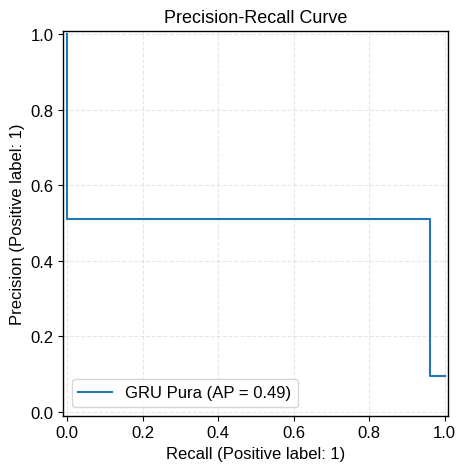
\includegraphics[width=0.7\textwidth]{figuras/modelos_resultados/gru/ap_gru_pior_fold.png} % insere o tikzpicture puro
  \label{fig:ap_gru_pior_fold}
  \legend{Fonte: Elaborado pelo autor.}
\end{figure}

Nesse gráfico, o \textit{baseline} não é fixo, mas igual a prevalência da classe positivos. No pior \textit{fold}, a proporção foi de aproximadamente
9,39\%, contrastando com o 49\% alcançado pelo modelo. Entretanto, a precisão foi baixa. Pelo gráfico, é possível ver que, por exemplo, seria 
possível ter um recall de 80\% porém com uma precisão menor que 60\%.

No melhor caso:

\begin{figure}[H]
  \centering
  \caption{Curva precisão vs \textit{recall} do modelo \ref{fig:gru_pura} em seu melhor \textit{fold}}
   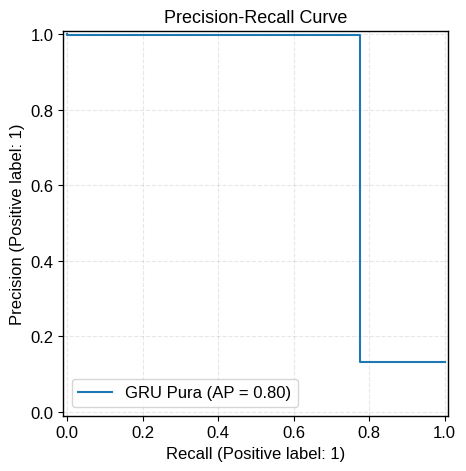
\includegraphics[width=0.7\textwidth]{figuras/modelos_resultados/gru/ap_gru_melhor_fold.png} % insere o tikzpicture puro
  \label{fig:ap_gru_melhor_fold}
  \legend{Fonte: Elaborado pelo autor.}
\end{figure}

Nesse \textit{fold}, o modelo alcançou um \textit{AP} de 80\%, enquanto que a proporção de casos positivos foi de 13,21\%. No melhor caso, 
entretanto, o modelo para ter 80\% de \textit{recall}, teria que baixar sua precisão para menos de 20\%. 

Apesar do desbalanceamento, o modelo alcançou resultados satisfatórios, considerando o extremo desbalanceamento do conjunto.

\section{Resultados do modelo híbrido GRU e CNN}
\label{sec:resultados_gru_cnn}

O modelo híbrido apresentou resultado superior em relação ao modelo descrito em \ref{fig:gru_pura}. Na tabela \ref{tab:resultado_cv_gru_cnn_validacao}
abaixo, é possível ver que o modelo obteve média maior em todas as métricas. Apesar disso, o modelo obteve um desvio padrão maior 
no \textit{recall} e \textit{F1-score}. 

\begin{table}[H]
\centering
\caption{Resultados do modelo híbrido CNN e GRU (\textit{N} vs. \textit{V}) na validação}
\label{tab:resultado_cv_gru_cnn_validacao}
\begin{tabular}{lcc}
\hline
\textbf{Métrica} & \textbf{Média} & \textbf{Desvio Padrão} \\
\hline
Precisão & 0.8800 &  0.1684 \\
\textit{Recall} & 0.8726  & 0.0857 \\
\textit{F1-Score} & 0.8593 & 0.0866 \\
Acurácia & 0.9730 & 0.0258 \\
\hline
\end{tabular}
\legend{Fonte: Elaborado pelo autor.}
\end{table}

Na tabela  \ref{tab:resultado_cv_gru_cnn_treino}, é possível observar que ainda há \textit{overfit} porém a diferença entre os resultados
do treino e validação do modelo \ref{fig:cnn_gru} é menor quando comparado com o modelo \ref{fig:gru_pura}. Por exemplo, a 
diferença percentual entre o \textit{f1-score} do primeiro modelo foi de aproximadamente 9,56\% enquanto que para o segundo, foi de, aproximadamente, 17,98\%

\begin{table}[H]
\centering
\caption{Resultados do modelo híbrido CNN e GRU (\textit{N} vs. \textit{V}) no treino}
\label{tab:resultado_cv_gru_cnn_treino}
\begin{tabular}{lcc}
\hline
\textbf{Métrica} & \textbf{Média} & \textbf{Desvio Padrão} \\
\hline
Precisão & 0.9698 &  0.0180 \\
\textit{Recall} & 0.9313  & 0.0268 \\
\textit{F1-Score} & 0.9502 & 0.0222\\
Acurácia & 0.9915 & 0.0035 \\
\hline
\end{tabular}
\legend{Fonte: Elaborado pelo autor.}
\end{table}

Na figura \ref{fig:gru_cnn_resultados_por_fold}, estão os resultados obtidos pelo modelo híbrido em cada \textit{fold}.

\begin{figure}[H]
  \centering
  \caption{Métricas do modelo híbrido CNN com GRU por \textit{fold}}
   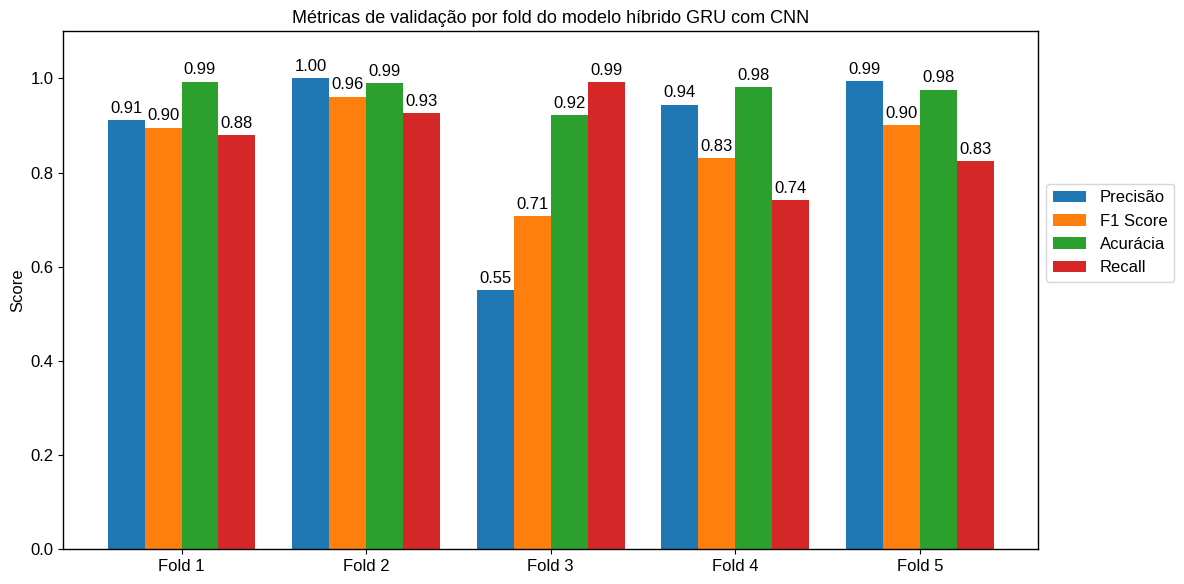
\includegraphics[width=1.0\textwidth]{figuras/modelos_resultados/gru_cnn/gru_cnn_metricas_por_fold.png} 
  \label{fig:gru_cnn_resultados_por_fold}
  \legend{Fonte: Elaborado pelo autor.}
\end{figure}

O modelo manteve a tendencia de ter uma precisão acima da acurácia na maioria dos \textit{folds}. É possível observar também que o modelo
obteve um \textit{recall} maior que o modelo GRU puro em todos os \textit{folds} e uma precisão, no geral, maior ou igual. Sendo as exceções,
os \textit{folds} quatro e cinco, porém a diferença foi de, aproximadamente, 0,01 pontos percentuais. 

A seguir, o desempenho do modelo em seu melhor e pior \textit{fold}. Repetindo os critérios descritos na seção \ref{sec:resultados_gru}, o melhor
\textit{fold} foi o segundo e o pior foi o terceiro.

Na figura \ref{fig:matriz_confusao_cnn_gru_melhor_fold}, é ilustrada a matriz de confusão do modelo em seu melhor \textit{fold}:

\begin{figure}[H]
  \centering
  \caption{Matriz de confusão modelo \ref{fig:cnn_gru} em seu melhor \textit{fold}}
   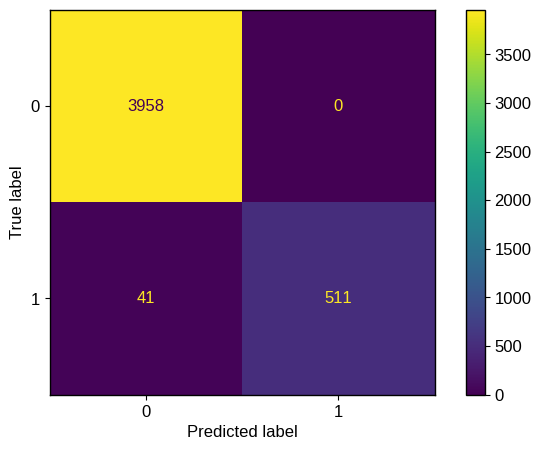
\includegraphics[width=0.7\textwidth]{figuras/modelos_resultados/gru_cnn/matriz_confusao_melhor_fold_gru_cnn_1_alt.png} 
  \label{fig:matriz_confusao_cnn_gru_melhor_fold}
  \legend{Fonte: Elaborado pelo autor.}
\end{figure}

Como pode ser visto no gráfico; o modelo não cometeu nenhum erro de falso positivo e errou 41 arritmias, classificando-as
como batimentos normais. 

Na matriz de confusão do pior \textit{fold}, ilustrado na figura \ref{fig:matriz_confusao_cnn_gru_pior_fold}, novamente,
a situação se inverte; a quantidade de erros de falsos negativos foi menor que as de falsos positivos, refletindo em um
\textit{recall} maior que a precisão; como pode ser observado no gráfico \ref{fig:gru_cnn_resultados_por_fold}.

\begin{figure}[H]
  \centering
  \caption{Matriz de confusão modelo \ref{fig:cnn_gru} em seu melhor \textit{fold}}
   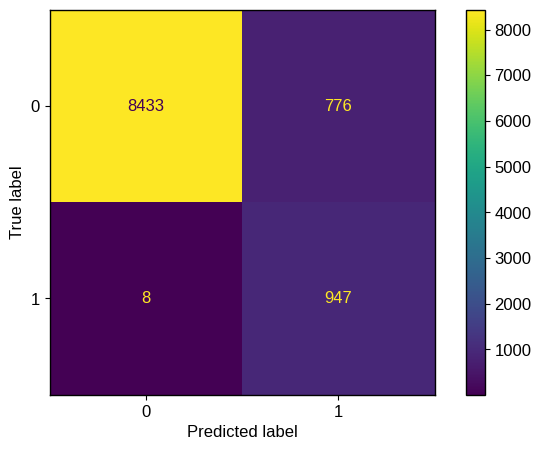
\includegraphics[width=0.7\textwidth]{figuras/modelos_resultados/gru_cnn/matriz_confusao_pior_fold_gru_cnn_3_alt.png} 
  \label{fig:matriz_confusao_cnn_gru_pior_fold}
  \legend{Fonte: Elaborado pelo autor.}
\end{figure}


No melhor, o modelo híbrido obteve um AP de 0,96, como pode ser visto na figura \ref{fig:roc_cnn_gru_melhor_fold}:


\begin{figure}[H]
  \centering
  \caption{Curva \textit{ROC} modelo \ref{fig:cnn_gru} em seu melhor \textit{fold}}
   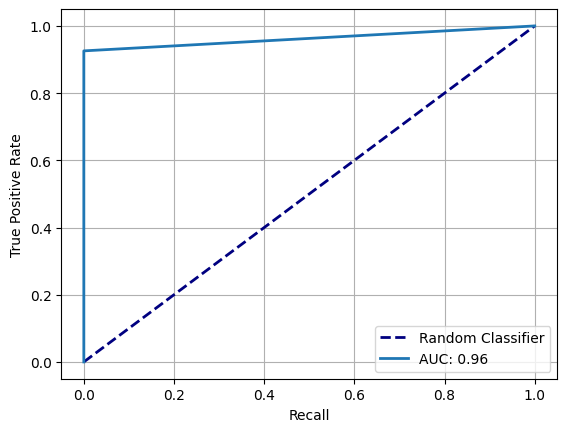
\includegraphics[width=0.7\textwidth]{figuras/modelos_resultados/gru_cnn/roc_cnn_melhor_fold_1.png} 
  \label{fig:roc_cnn_gru_melhor_fold}
  \legend{Fonte: Elaborado pelo autor.}
\end{figure}

Considerando a curva PR, o AP também foi maior:

\begin{figure}[H]
  \centering
  \caption{Curva precisão vs \textit{recall} do modelo \ref{fig:cnn_gru} em seu melhor \textit{fold}}
   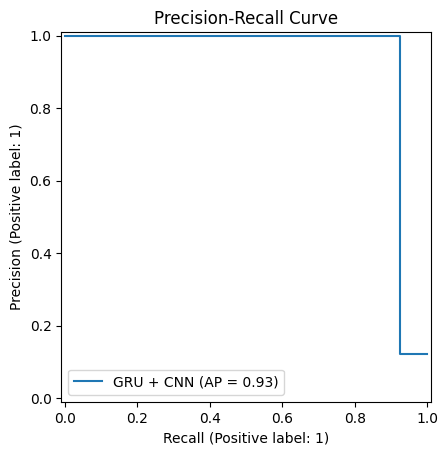
\includegraphics[width=0.7\textwidth]{figuras/modelos_resultados/gru_cnn/ap_gru_cnn_melhor_fold_1.png} 
  \label{fig:ap_cnn_gru_melhor_fold}
  \legend{Fonte: Elaborado pelo autor.}
\end{figure}

Pelo gráfico \ref{fig:ap_cnn_gru_melhor_fold}, nesse \textit{fold}, o modelo conseguiria manter um \textit{recall} de até 80\%
enquanto sua precisão permanece em torno de quase 100\%, desempenho superior ao modelo GRU puro.

A curva \textit{ROC} desse modelo no pior \textit{fold} é descrita a seguir:

\begin{figure}[H]
  \centering
  \caption{Curva \textit{ROC} modelo \ref{fig:cnn_gru} em seu pior \textit{fold}}
   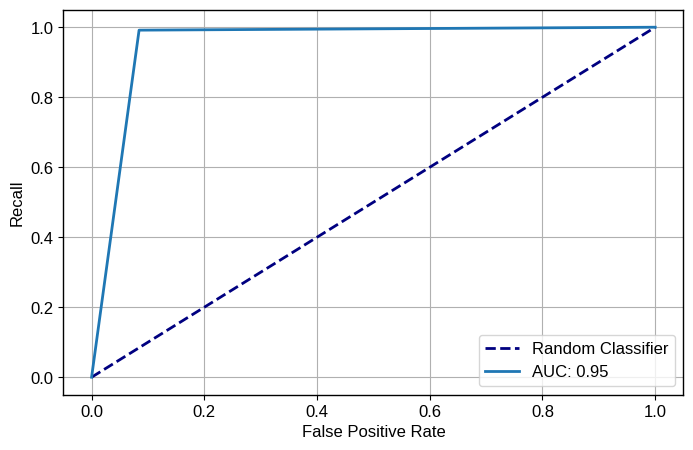
\includegraphics[width=0.7\textwidth]{figuras/modelos_resultados/gru_cnn/roc_cnn_pior_fold_3.png} 
  \label{fig:roc_cnn_gru_pior_fold}
  \legend{Fonte: Elaborado pelo autor.}
\end{figure}

O AP foi de 0,87, igual ao obtido no modelo GRU puro. Já a curva PR descrita na figura

\begin{figure}[H]
  \centering
  \caption{Curva precisão vs \textit{recall} do modelo \ref{fig:cnn_gru} em seu melhor \textit{fold}}
   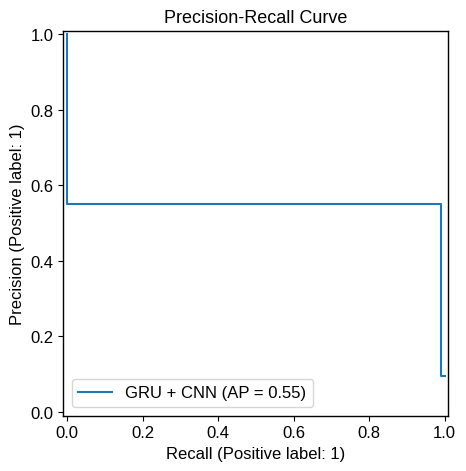
\includegraphics[width=0.7\textwidth]{figuras/modelos_resultados/gru_cnn/ap_gru_cnn_pior_fold_3.png} 
  \label{fig:ap_cnn_gru_pior_fold}
  \legend{Fonte: Elaborado pelo autor.}
\end{figure}

Nesse cenário, o modelo conseguiria manter um \textit{recall} de até 80\% com um pouco menos de 60\% de precisão.

De modo geral, os modelos exibiram um perfil semelhante em seu pior e melhor caso. No pior, a sensibilidade foi maior, resultados
em maiores erros de falso positivo, como resultado, o \textit{recall} foi alto e a precisão foi baixa. No melhor caso, houve um 
equilíbrio maior e, apesar do \textit{recall} mais baixo, a alta precisão aumentou o \textit{f1-score}.

Em contextos médicos, é preferível um \textit{recall} maior, pois falsos negativos são mais danosos que um falso positivo; isto é, é melhor
dizer que um batimento normal é arrítmico do que o contrário. Entretanto, uma precisão muito baixa pode indicar que o modelo é 
tão bom quanto um modelo aleatório; o que o tornaria inútil. 

Como evidenciado pelo AP, ambos os modelos se saíram bem melhor do que esse \textit{baseline}.

\chapter{Análise de erros no pior \textit{fold}}
\label{ch:analise_erros_pior_fold}

Pelos critérios adotados, o terceiro fold foi o de pior desempenho em ambos os modelos.
Como o recall foi superior à precisão, supõe-se que a causa esteja relacionada à presença de batimentos normais com características morfológicas atípicas, o que pode ter confundido os modelos.
Para fins de ilustração, apresenta-se a seguir uma breve análise de erros do desempenho do melhor modelo em seu cenário mais desafiador.
Devido a essa limitação, os resultados discutidos não permitem conclusões generalizáveis, servindo apenas como apoio à interpretação dos achados.

\section{Análise de erros do modelo híbrido CNN com GRU}
\label{sec:analise_erros_cnn_gru}

Na tabela \ref{tab:erros_acertos_por_paciente} a seguir, é possível ver que a maioria dos erros foi oriunda de um paciente, o 203.

\begin{table}[H]
\centering
\caption{Total dos erros e acertos por paciente no \textit{fold} de validação}
\label{tab:erros_acertos_por_paciente}
\begin{tabular}{lcc}
\hline
\textbf{Pacientes} & \textbf{Erros} & \textbf{Acertos}\\
\hline
119 & 0 &  1972 \\
203 & 772  & 2186\\
205 & 11 & 2616\\
209 & 1 & 2606\\
\hline
\end{tabular}
\legend{Fonte: Elaborado pelo autor.}
\end{table}

Aproximadamente, 98,46\% de todos os erros foram desse paciente. O modelo errou em torno de 35,31\% de seus batimentos. Conforme visto na 
figura \ref{fig:matriz_confusao_cnn_gru_pior_fold}, a maioria desses erros são de falsos positivos.

Segundo as anotações do MIT-BIH, disponíveis em \cite{physionet_annotations}, o paciente 203 é considerado como muito difícil. As anotações ainda citam
a presença de mudança de morfologia no complexo QRS e contrações ventriculares prematuras (PVC) de múltiplas formas.

Na figura \ref{fig:matriz_confusao_paciente_mais_dificil}, é mostrada a matriz de confusão desse paciente.

\begin{figure}[H]
  \centering
  \caption{Matriz de confusão do paciente 203}
   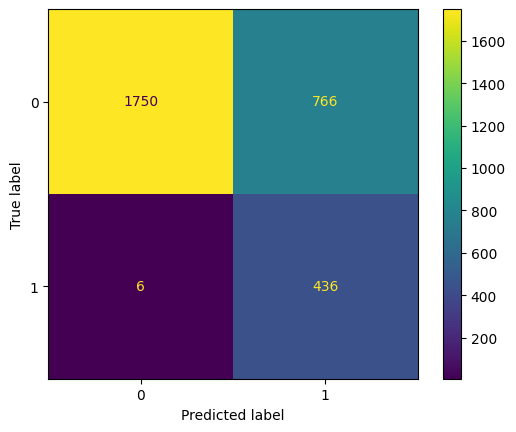
\includegraphics[width=0.7\textwidth]{figuras/analise_erros/matriz_confusao_paciente_mais_dificil.png} 
  \label{fig:matriz_confusao_paciente_mais_dificil}
  \legend{Fonte: Elaborado pelo autor.}
\end{figure}

O modelo confundiu seis batimentos ventriculares como normais e 766 normais como ventriculares. Na figura
\ref{fig:erro_acert_neg_class_paciente_mais_dificil}, é ilustrado duas sequencias desse paciente, na primeira
uma sequencia normal classificada como arrítmica e na segunda uma normal corretamente classificada.

\begin{figure}[H]
  \centering
  \caption{ECG normal do paciente 203: erro e acerto}
   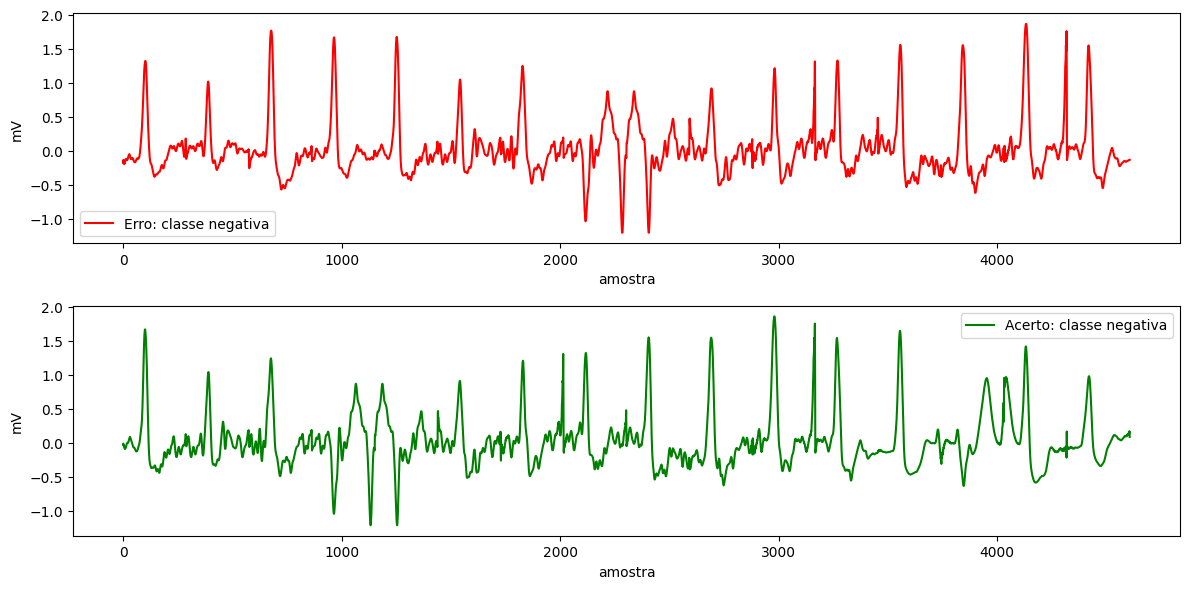
\includegraphics[width=1.0\textwidth]{figuras/analise_erros/ecg_erro_acerto_neg_paciente_mais_dificil.png} 
  \label{fig:erro_acert_neg_class_paciente_mais_dificil}
  \legend{Fonte: Elaborado pelo autor.}
\end{figure}

É possível observar a forte presença de ruído em ambos os casos. E a presença de batimentos com a morfologia 
bem deformada; após a amostra 2000 no primeiro gráfico e após a amostra 1000 no segundo.

Para comparação, na figura \ref{fig:acert_neg_class_paciente_mais_facil}, paciente para o qual o modelo não cometeu erros,
abaixo é ilustrado uma sequência normal.

\begin{figure}[H]
  \centering
  \caption{ECG normal do paciente 119.}
   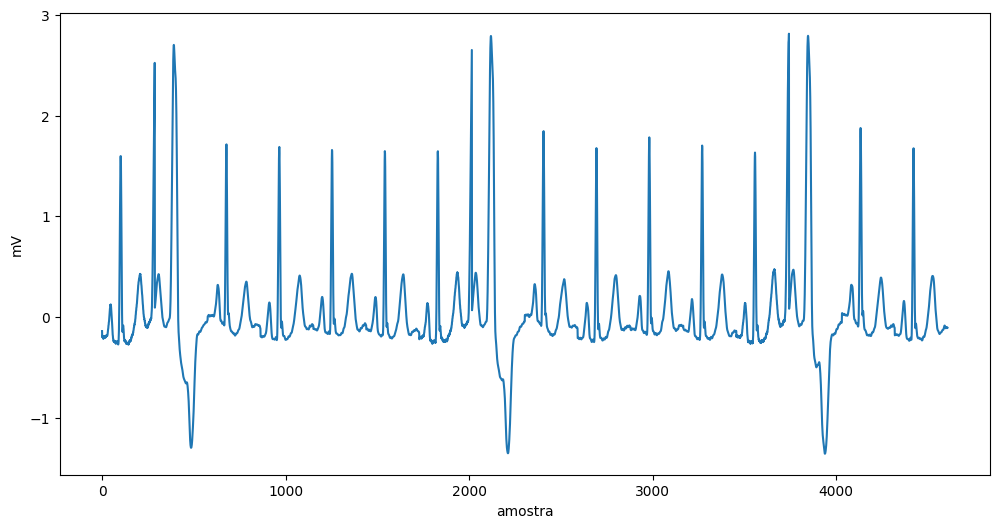
\includegraphics[width=1.0\textwidth]{figuras/analise_erros/ecg_sequencia_normal_neg_paciente_mais_facil.png} 
  \label{fig:acert_neg_class_paciente_mais_facil}
  \legend{Fonte: Elaborado pelo autor.}
\end{figure}

É possível notar uma sequencia mais limpa e com o complexo QRS com morfologia usual. Note em torno da amostra
2000 uma contração prematura ventricular usual.

Na figura \ref{fig:erro_acert_pos_class_paciente_mais_dificil} é ilustrado duas sequências arrítmicas do paciente 203, a primeiro o modelo acertou e a segunda ele errou:

Em ambos os casos, é observável o ruído presenta na figura \ref{fig:erro_acert_neg_class_paciente_mais_dificil}. O 
último batimento da sequência também apresenta uma morfologia diferente da usual.

\begin{figure}[H]
  \centering
  \caption{ECG normal do paciente 203: acerto e erro}
   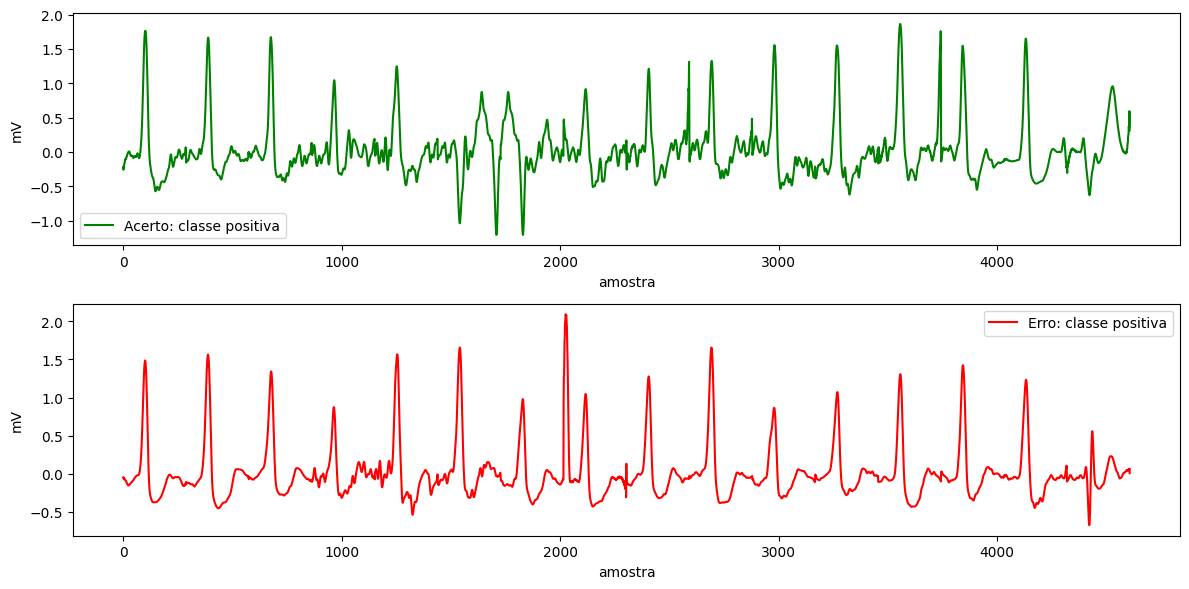
\includegraphics[width=1.0\textwidth]{figuras/analise_erros/ecg_erro_acerto_pos_paciente_mais_dificil.png} 
  \label{fig:erro_acert_pos_class_paciente_mais_dificil}
  \legend{Fonte: Elaborado pelo autor.}
\end{figure}

Já na figura \ref{fig:acert_posclass_paciente_mais_facil}, é ilustrada uma sequencia arrítmica do paciente 119.
Observe no último batimento, uma arritmia ventricular com uma forma bem definida.

\begin{figure}[H]
  \centering
  \caption{ECG arrítmico do paciente 119.}
   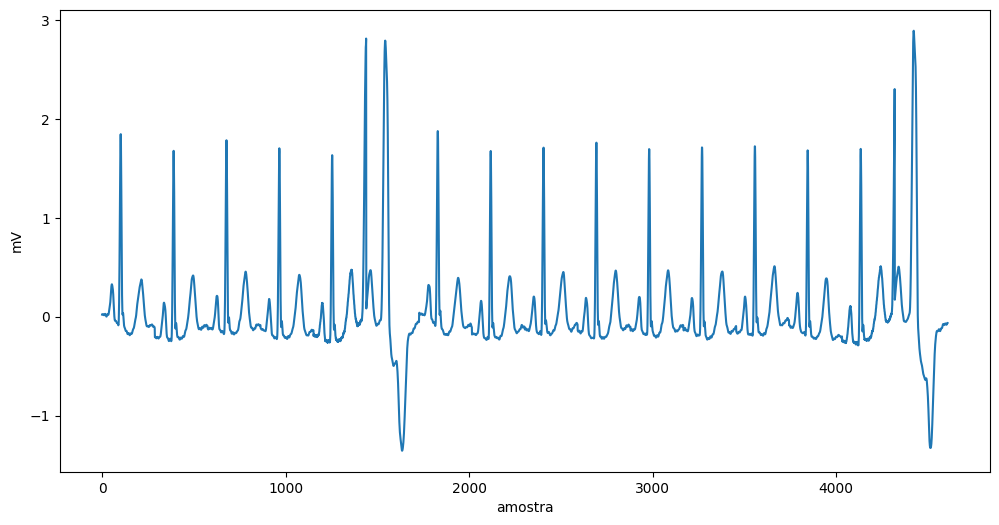
\includegraphics[width=1.0\textwidth]{figuras/analise_erros/ecg_sequencia_normal_pos_paciente_mais_facil.png} 
  \label{fig:acert_posclass_paciente_mais_facil}
  \legend{Fonte: Elaborado pelo autor.}
\end{figure}

Apesar das diferenças naturais entre ECGs de pacientes diferentes, pelo o que foi visto no gráfico e o que está registrado
nas anotações do MIT-BIH; o ECG desse paciente possui muito ruído e QRS com morfologia mais diferente, especialmente
quando comparando com as do paciente 119; essas diferenças pode ter levado o modelo ao erro. Apesar de que, por ser 
pouca interpretabilidade, não é possível fazer uma afirmação.

